\documentclass[14pt]{beamer}
\usepackage[T2A]{fontenc}
\usepackage{verbatim}
\usepackage[utf8]{inputenc}
\usepackage[english,russian]{babel}
\usepackage{amssymb,amsfonts,amsmath,mathtext}
\usepackage{cite,enumerate,float,indentfirst}
\usepackage{multirow}

\graphicspath{{images/}}

\usetheme{Pittsburgh}
\usecolortheme{whale}

\setbeamercolor{footline}{fg=blue}
\setbeamertemplate{footline}{
  \leavevmode%
  \hbox{%
  \begin{beamercolorbox}[wd=.333333\paperwidth,ht=2.25ex,dp=1ex,center]{}%
    Е. Б. Анюшева, МФТИ
  \end{beamercolorbox}%
  \begin{beamercolorbox}[wd=.333333\paperwidth,ht=2.25ex,dp=1ex,center]{}%
    Москва, 2019
  \end{beamercolorbox}%
  \begin{beamercolorbox}[wd=.333333\paperwidth,ht=2.25ex,dp=1ex,right]{}%
  Стр. \insertframenumber{} из \inserttotalframenumber \hspace*{2ex}
  \end{beamercolorbox}}%
  \vskip0pt%
}

\newcommand{\itemi}{\item[\checkmark]}

\title{\small{Верификация доказательства теоремы о нижней оценке хроматического числа плоскости в системе {\tt Coq} }}
\author{\small{%
\emph{Выступающий:}~Е.Б.Анюшева\\%
\emph{Руководитель:}~к.ф.-м.н.~Е.В.Дашков}\\%
\vspace{30pt}%
Факультет Инноваций и Высоких Технологий \\
МФТИ (ГУ)%
\vspace{20pt}%
}
\date{\small{Москва, 2019}}

\begin{document}

\maketitle


\begin{frame}
\center{Полный исходный код находится по адресу}
\center{\href{https://github.com/LenaAn/deGrey_proofs}{https://github.com/LenaAn/deGrey\_proofs}}
\end{frame}

\begin{frame}
\frametitle{Задача \\о хроматическом числе плоскости}

\begin{figure}[h]
  \begin{minipage}[h]{0.49\linewidth}
    \center{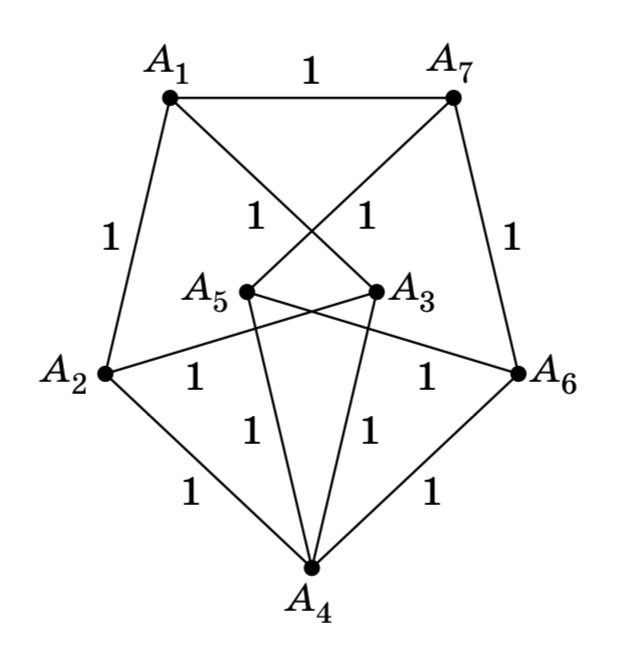
\includegraphics[height=7\baselineskip,width=1\linewidth]{Moser_Spindle.png}}
    $$\chi \ge 4 $$ \\  1950 год
  \end{minipage}
  \hfill
  \begin{minipage}[h]{0.49\linewidth}
    \center{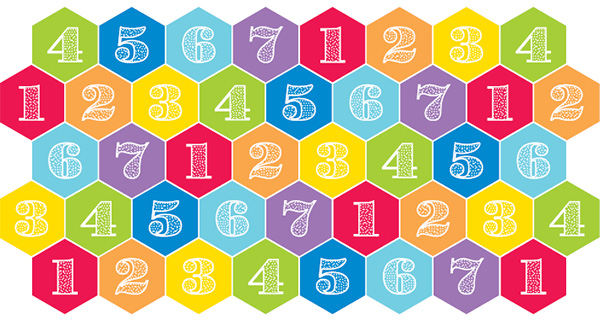
\includegraphics[height=7\baselineskip,width=1\linewidth]{raskraska7}}
    $$\chi \le 7 $$ \\ 1950 год
  \end{minipage}
\end{figure}
\end{frame}

\begin{frame}
\frametitle{Хроматическое число плоскости \\ не меньше 5}

\begin{figure}[h]
  \begin{minipage}[h]{0.2\linewidth}
    \center{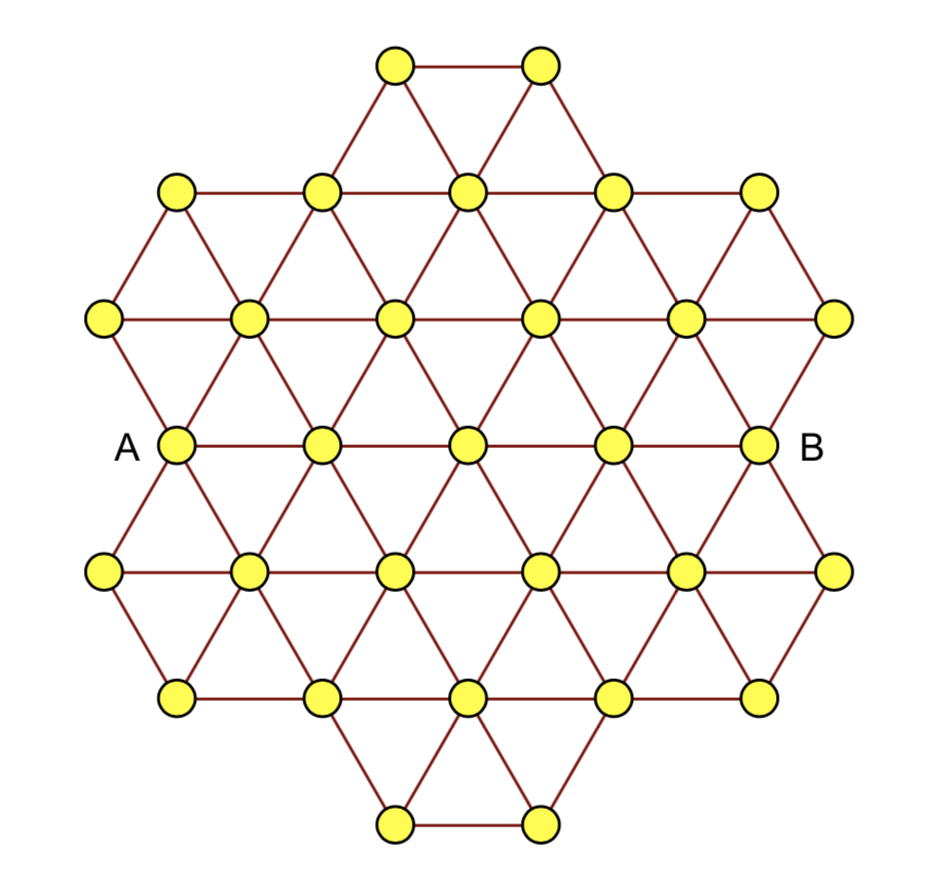
\includegraphics[width=1\linewidth]{Graph_J}}
    Граф $J$
  \end{minipage}
  \begin{minipage}[h]{0.05\linewidth}
  \vspace{-1cm}$$\to $$
  \end{minipage}
  \begin{minipage}[h]{0.2\linewidth}
    \center{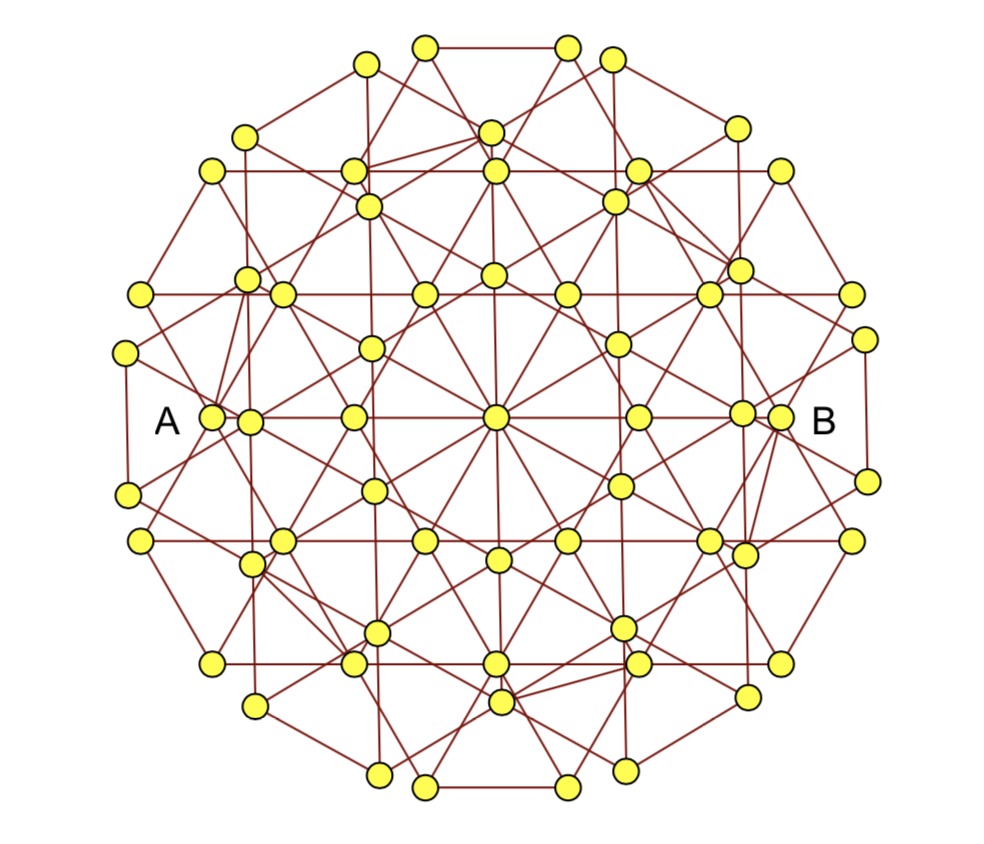
\includegraphics[width=1\linewidth]{Graph_K}}
    Граф $K$
  \end{minipage}
  \begin{minipage}[h]{0.05\linewidth}
  \vspace{-1cm}$$\to $$
  \end{minipage}
  \begin{minipage}[h]{0.2\linewidth}
    \center{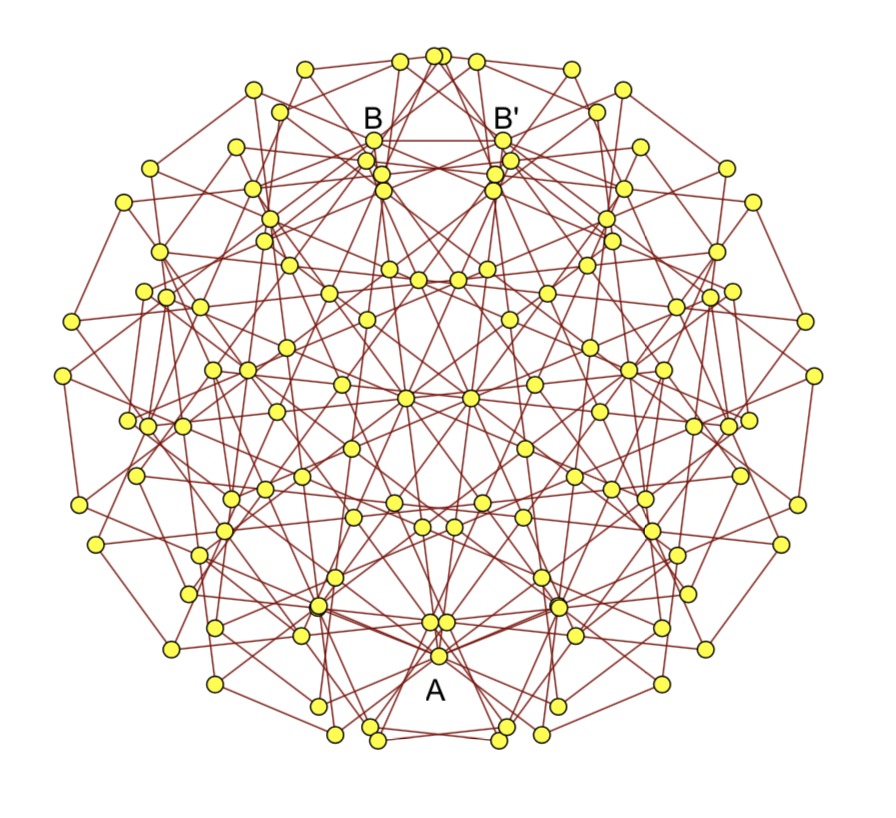
\includegraphics[width=1\linewidth]{Graph_L}}
    Граф $L$
  \end{minipage}
\end{figure}

\hrule

\begin{figure}[h]
  \begin{minipage}[h]{0.2\linewidth}
    \center{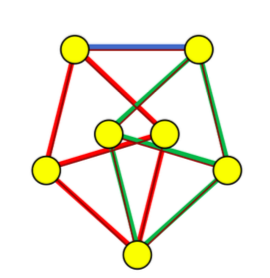
\includegraphics[width=1\linewidth]{Spindle.png}}
    Веретено
  \end{minipage}
  \begin{minipage}[h]{0.03\linewidth}
  \vspace{-1cm}$$\to $$
  \end{minipage}
  \begin{minipage}[h]{0.2\linewidth}
    \center{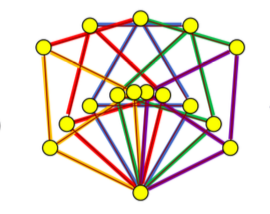
\includegraphics[width=1\linewidth]{Spindles.png}}
    Веретена
  \end{minipage}
  \begin{minipage}[h]{0.03\linewidth}
  \vspace{-1cm}$$\to $$
  \end{minipage}
  \begin{minipage}[h]{0.2\linewidth}
    \center{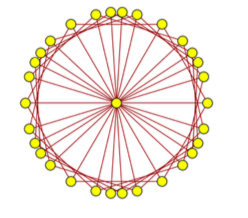
\includegraphics[width=1\linewidth]{Graph_V.png}}
    Граф V
  \end{minipage}
  \begin{minipage}[h]{0.03\linewidth}
  \vspace{-1cm}$$\to $$
  \end{minipage}
  \hfill
  \begin{minipage}[h]{0.2\linewidth}
  {\small Граф $N$ \\ с $20425$ \\  вершинами}
  \end{minipage}
\end{figure}
\end{frame}

\begin{frame}
\frametitle{Текущее состояние задачи: \\ верификация с помощью SAT-solver'а}
\begin{itemize}
    \item Найден меньший пример графа, не раскрашиваемого в $4$ цвета, он имеет $1585$ вершин
    \item Утверждение о том, что данный граф не раскрашивается в $4$ цвета, записано в виде формулы первого порядка и сведено в задаче SAT
    \item С помощью SAT-solver'а проверено отсутствие раскраски в $4$ цвета
\end{itemize}
\end{frame}

\begin{frame}
\frametitle{Цели работы}
\begin{itemize}
    \item Разработка методов конструкций графов в системе {\tt Coq}
    \item Формализация конструкций графов
    \item формализация утверждений статьи в системе {\tt Coq}
    \item Верификация утверждений статьи
\end{itemize}
\end{frame}

\begin{frame}
\frametitle{Система {\tt Coq}}
\begin{itemize}
    \item Система для {\it верификации} доказательств теорем
    \item Использует {\it Исчесление индуктивных конструкций (Calculus of Inductive Constructions) }
    \item {\it Соответствие Карри-Ховарда }
    \begin{tabular}{cc}
    Теорема & Терм \\
    Утверждение & Тип \\
    Доказательство & Терм данного типа
\end{tabular}
\end{itemize}
\end{frame}

\begin{frame}
\frametitle{Актуальность компьютерной верификации }
\begin{itemize}
    \item Структура данных с несвязным множеством: доказательство корректности в {\tt Coq} было опубликовано в 2007 году.
    \item Теорема Фейта – Томпсона: формальное доказательство с использованием {\tt Coq} было завершено в сентябре 2012 года.
    \item Теорема о четырех цветах: формальное доказательство с использованием {\tt Coq} было завершено в 2005 году.
\end{itemize}
\end{frame}

\begin{frame}[fragile]
\frametitle{Представление графов в {\tt Coq}}

\begin{verbatim}
Definition node := PositiveOrderedTypeBits.t.
Definition nodeset := PositiveSet.t.
Definition nodemap: Type -> Type :=
                        PositiveMap.t.
Definition graph := nodemap nodeset.
\end{verbatim} 

\end{frame}

\begin{frame}[fragile]
\frametitle{Представление графов в {\tt Coq}}
\begin{figure}[h]
  \begin{minipage}[h]{1\linewidth}
    \center{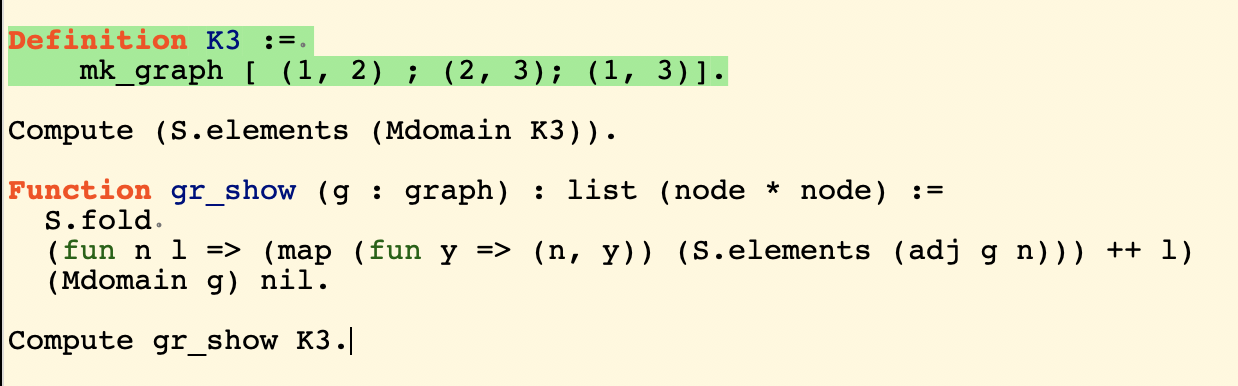
\includegraphics[width=1\linewidth]{Step2.png}}
  \end{minipage}
\end{figure}
\hrule
\begin{figure}[h]
  \begin{minipage}[h]{1\linewidth}
    \center{
\includegraphics[width=1\linewidth]{Res2.png}}
  \end{minipage}
\end{figure}
\end{frame}

\begin{frame}[fragile]
\frametitle{Представление графов в {\tt Coq}}
\begin{figure}[h]
  \begin{minipage}[h]{1\linewidth}
    \center{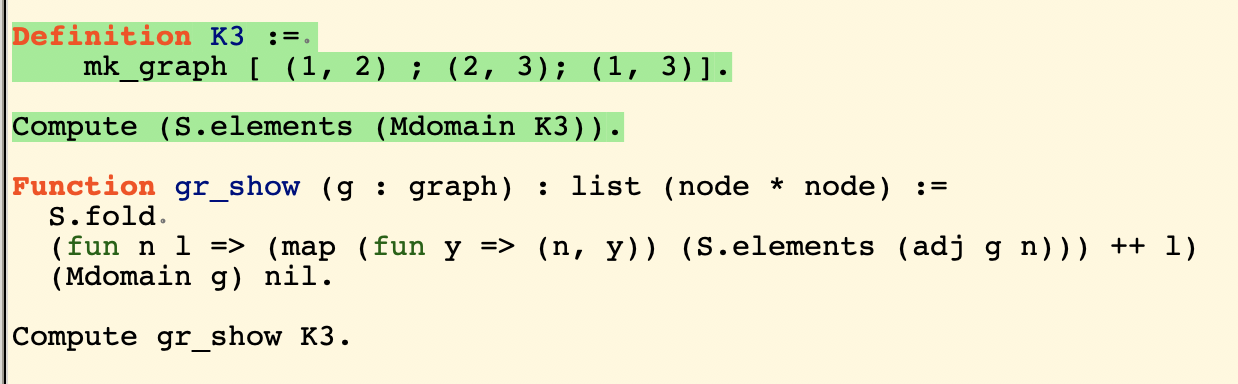
\includegraphics[width=1\linewidth]{Step3.png}}
  \end{minipage}
\end{figure}
\hrule
\begin{figure}[h]
  \begin{minipage}[h]{1\linewidth}
    \center{
\includegraphics[width=1\linewidth]{Res3.png}}
  \end{minipage}
\end{figure}
\end{frame}

\begin{frame}[fragile]
\frametitle{Представление графов в {\tt Coq}}
\begin{figure}[h]
  \begin{minipage}[h]{1\linewidth}
    \center{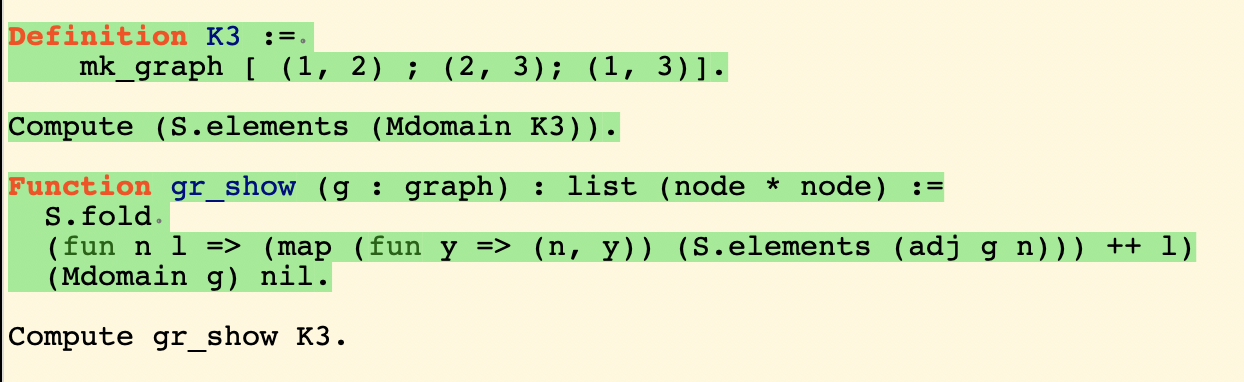
\includegraphics[width=1\linewidth]{Step4.png}}
  \end{minipage}
\end{figure}
\hrule
\begin{figure}[h]
  \begin{minipage}[h]{1\linewidth}
    \center{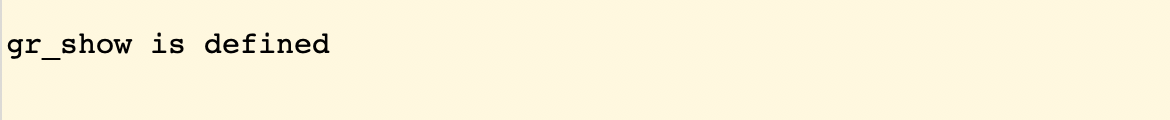
\includegraphics[width=1\linewidth]{Res4.png}}
  \end{minipage}
\end{figure}

\end{frame}

\begin{frame}[fragile]
\frametitle{Представление графов в {\tt Coq}}
\begin{figure}[h]
  \begin{minipage}[h]{1\linewidth}
    \center{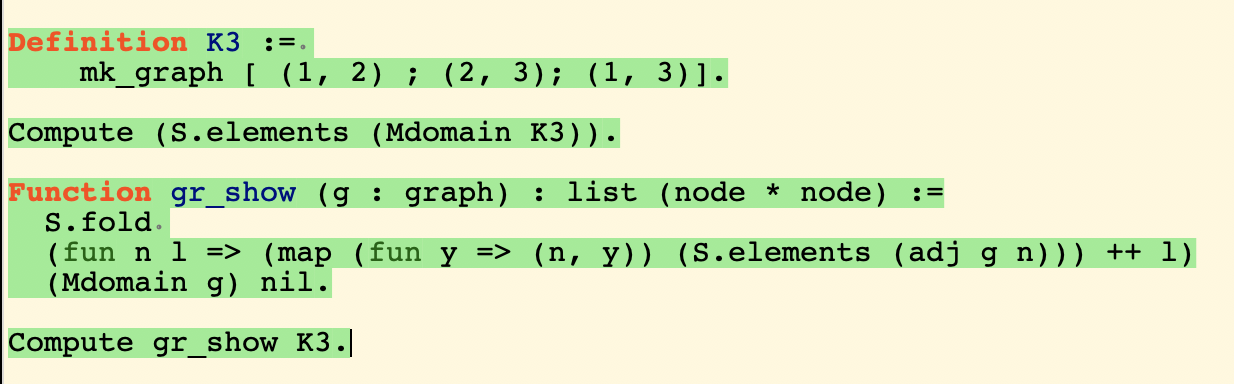
\includegraphics[width=1\linewidth]{Step5.png}}
  \end{minipage}
\end{figure}
\hrule
\begin{figure}[h]
  \begin{minipage}[h]{1\linewidth}
    \center{
\includegraphics[width=1\linewidth]{Res5.png}}
  \end{minipage}
\end{figure}

\end{frame}

\begin{frame}[fragile]
\frametitle{Представление графов в {\tt Coq}}

{\small 
\begin{verbatim}
Definition add_edge (e: (E.t*E.t)) (g: graph) : 
                                        graph :=
 M.add (fst e) (S.add (snd e) (adj g (fst e))) 
  (M.add (snd e) (S.add (fst e) (adj g (snd e))) g).
\end{verbatim}
}

\begin{verbatim}
Definition mk_graph (el: list (E.t*E.t)) :=
  fold_right add_edge (M.empty _) el.
\end{verbatim}

\begin{verbatim}
Definition K3 := 
    mk_graph [(1, 2); (2, 3); (1, 3)].
\end{verbatim}
\end{frame}

\begin{frame}[fragile]
\frametitle{Представление графов в {\tt Coq}: функции}
Функции для работы с графами с высокой степенью симметрии:
\begin{itemize}
    \item {\tt l\_rng (l : list node) : node * node}
    \item {\tt gr\_rng (g : graph) : node * node}
    \item {\tt rename\_all (f : node -> node) (g : graph) : graph}
    \item {\tt delete\_edge (g: graph) (a b : node) : graph}
    \item {\tt rename\_in\_order (g: graph) : graph}
    \item {\tt mk\_cmn\_edge (g1 g2 : graph) (a b n m : node) : graph}
\end{itemize}
\end{frame}

\begin{frame}[fragile]
\frametitle{Представление графов в {\tt Coq}: граф {\tt H}}

{\small 
\begin{verbatim}
Definition H : graph := 
  let g1 := rename_in_order 
    (mk_cmn_edge K3 K3 1 3 1 3) in
  let g2 := rename_in_order 
    (mk_cmn_edge g1 K3 1 (snd (gr_rng g1)) 1 3) in
  let g3 := rename_in_order 
    (mk_cmn_edge g2 K3 1 (snd (gr_rng g2)) 1 3) in
  let g4 := rename_in_order 
    (mk_cmn_edge g3 K3 1 (snd (gr_rng g3)) 1 3) in
  rename_in_order 
    (add_edge (2, snd (gr_rng g4)) g4).
\end{verbatim}
}
\end{frame}

\begin{frame}[fragile]
\frametitle{Представление графов в {\tt Coq}: граф {\tt J}}

{\small 
\begin{verbatim}
Definition J: graph :=
  let HH := mk_cmn_edge H H 2 3 6 7 in
  let HH_H := mk_cmn_edge HH H 7 2 6 7 in
  let HHH := rename_node 14 12 HH_H in
  let HHH_H := mk_cmn_edge HHH H 6 7 6 7 in
  let HHHH := rename_node 19 17 HHH_H in
  let HHHH_H := mk_cmn_edge HHHH H 5 6 6 7 in
  let HHHHH := rename_node 24 22 HHHH_H in
  let HHHHH_H := mk_cmn_edge HHHHH H 4 5 6 7 in
  let HHHHHH := rename_node 29 27 HHHHH_H in
  let HHHHHH_H := mk_cmn_edge HHHHHH H 3 4 6 7 in
  let HHHHHHH :=  rename_node 34 32 HHHHHH_H in
  rename_in_order (rename_node 37 9 HHHHHHH).
\end{verbatim}
}
\end{frame}

\begin{frame}[fragile]
\frametitle{Представление графов в {\tt Coq}: \\ графы {\tt K} и {\tt L}}

{\small 
\begin{verbatim}
Definition K: graph :=
  let JJ := mk_art J J 1 1 in
  let JJ := add_edges [
            (9, 9+31); (12, 12+31); (16, 16+31); 
            (20, 20+31); (24, 24+31); (28, 28+31)
            ] JJ in
  rename_in_order JJ.

Definition L: graph :=
  let KK := mk_art K K A A in
  let KK := add_edge (B, B+snd(gr_rng K)) KK in
  rename_in_order KK.
\end{verbatim}
}
\end{frame}

\begin{frame}[fragile]
\frametitle{Доказательства корректности \\ операций над графами}

\begin{verbatim}
Definition undirected (g: graph) := 
   forall i j, S.In j (adj g i) -> 
                        S.In i (adj g j).

Definition no_selfloop (g: graph) := 
    forall i, ~ S.In i (adj g i).

Definition graph_ok (g : graph) := 
  undirected g /\ no_selfloop g.
\end{verbatim}
\end{frame}

\begin{frame}[fragile]
\frametitle{Доказательства корректности \\ операций над графами: {\tt H\_ok}}

\begin{figure}[h]
  \begin{minipage}[h]{1\linewidth}
    \center{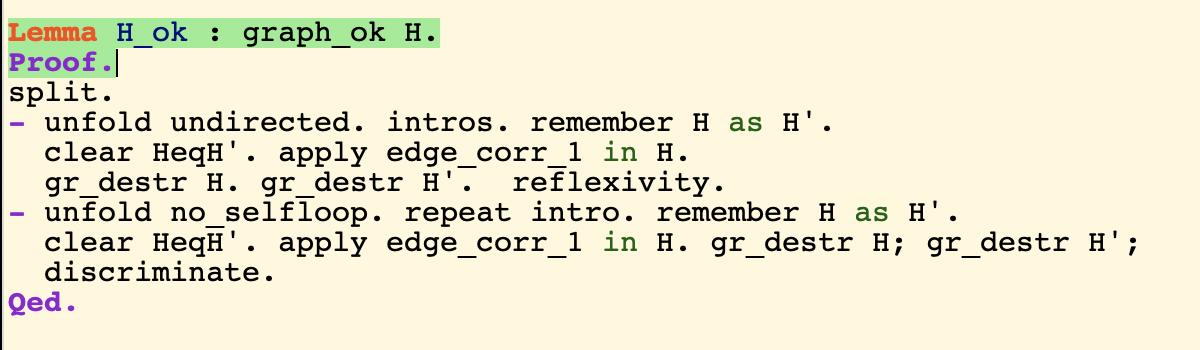
\includegraphics[width=1\linewidth]{H_ok1.png}}
  \end{minipage}
  \begin{minipage}[h]{1\linewidth}
    \center{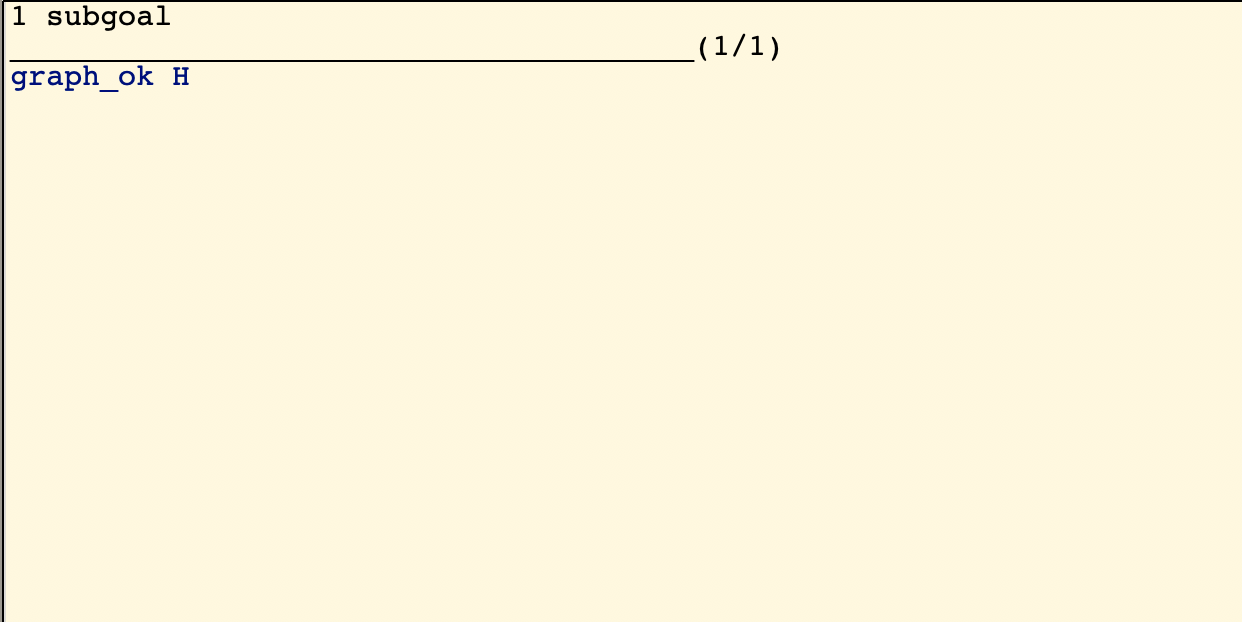
\includegraphics[width=1\linewidth]{context1.png}}
  \end{minipage}
\end{figure}
\end{frame}

\begin{frame}[fragile]
\frametitle{Доказательства корректности \\ операций над графами: {\tt H\_ok}}

\begin{figure}[h]
  \begin{minipage}[h]{1\linewidth}
    \center{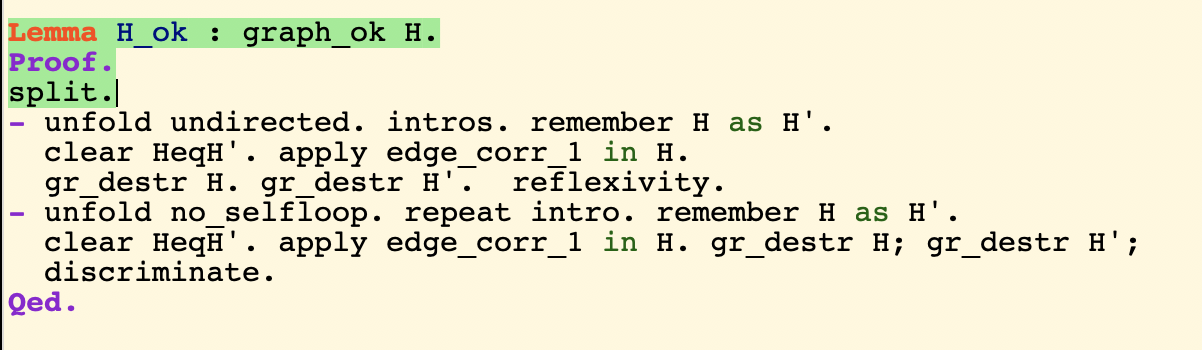
\includegraphics[width=1\linewidth]{H-ok2.png}}
  \end{minipage}
  \begin{minipage}[h]{1\linewidth}
    \center{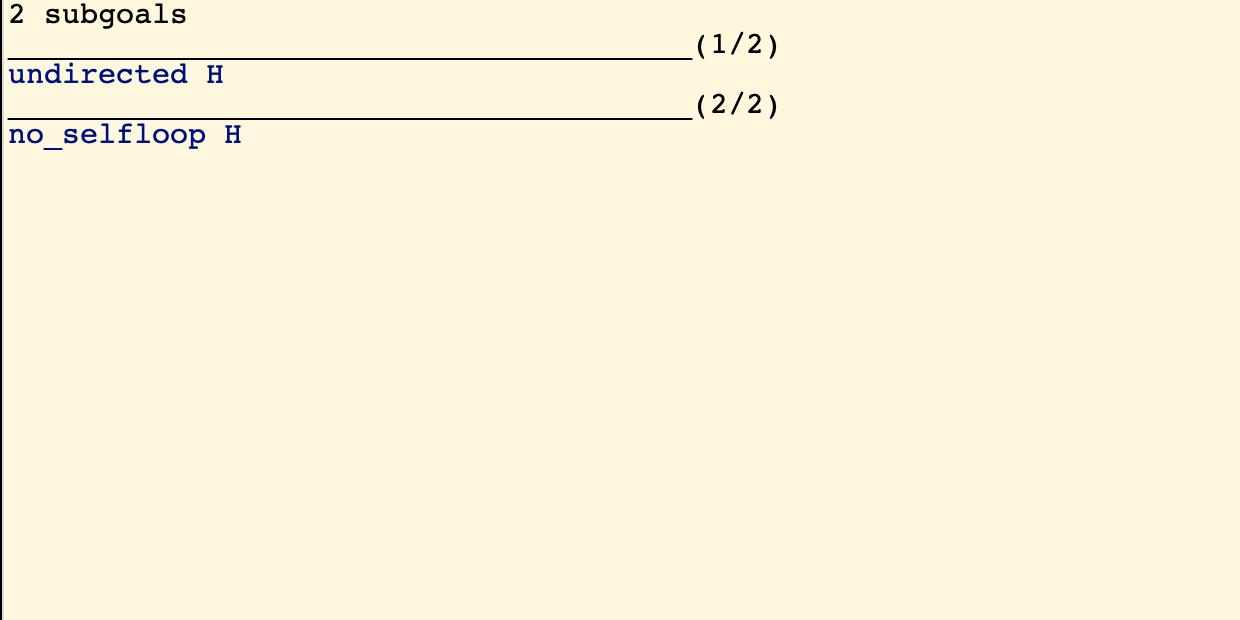
\includegraphics[width=1\linewidth]{context2.png}}
  \end{minipage}
\end{figure}
\end{frame}

\begin{frame}[fragile]
\frametitle{Доказательства корректности \\ операций над графами: {\tt H\_ok}}

\begin{figure}[h]
  \begin{minipage}[h]{1\linewidth}
    \center{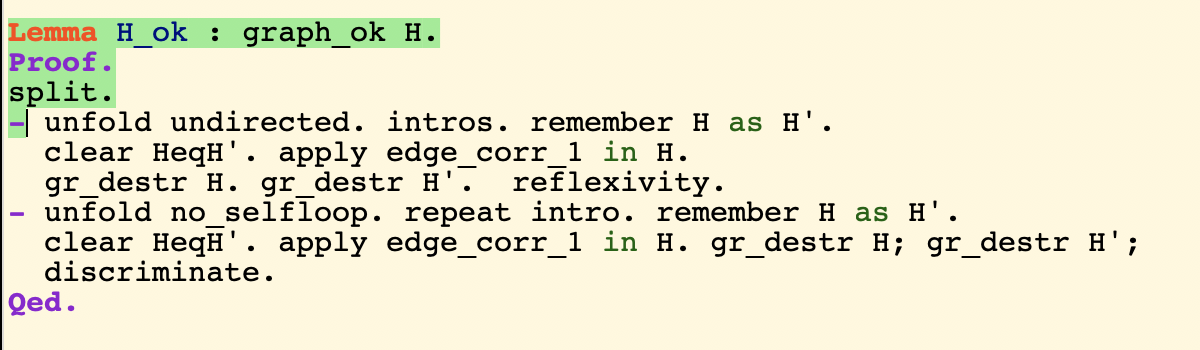
\includegraphics[width=1\linewidth]{H-ok3.png}}
  \end{minipage}
  \begin{minipage}[h]{1\linewidth}
    \center{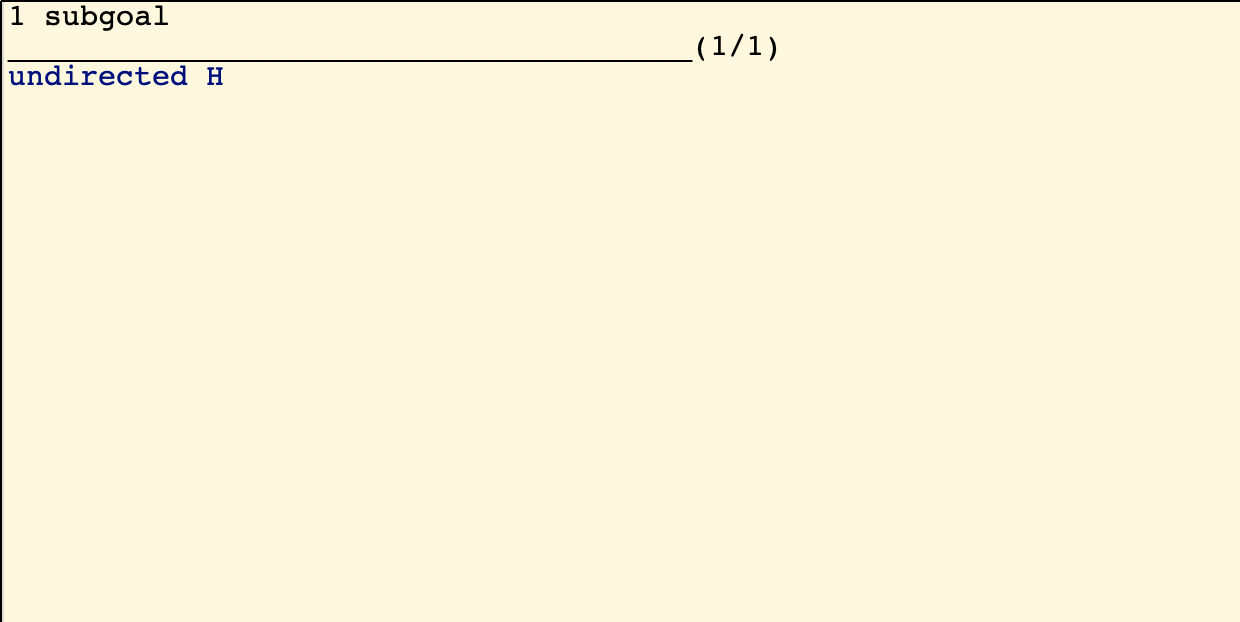
\includegraphics[width=1\linewidth]{context3.png}}
  \end{minipage}
\end{figure}
\end{frame}

\begin{frame}[fragile]
\frametitle{Доказательства корректности \\ операций над графами: {\tt H\_ok}}

\begin{figure}[h]
  \begin{minipage}[h]{1\linewidth}
    \center{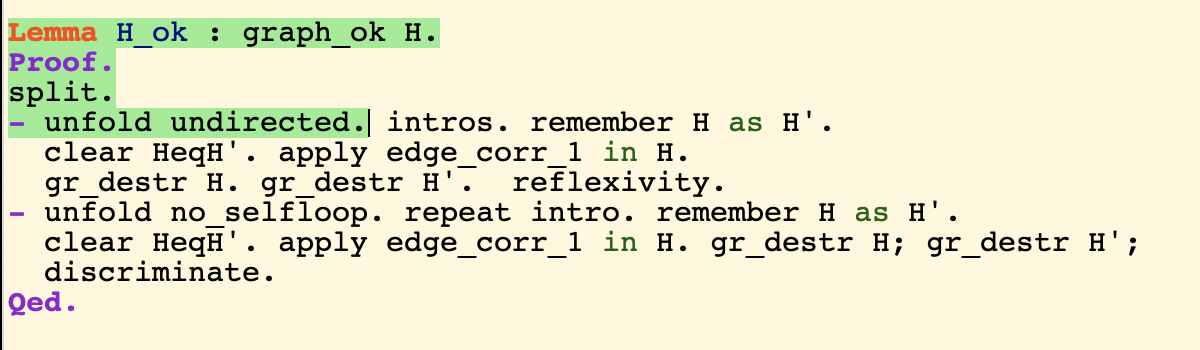
\includegraphics[width=1\linewidth]{H-ok4.png}}
  \end{minipage}
  \begin{minipage}[h]{1\linewidth}
    \center{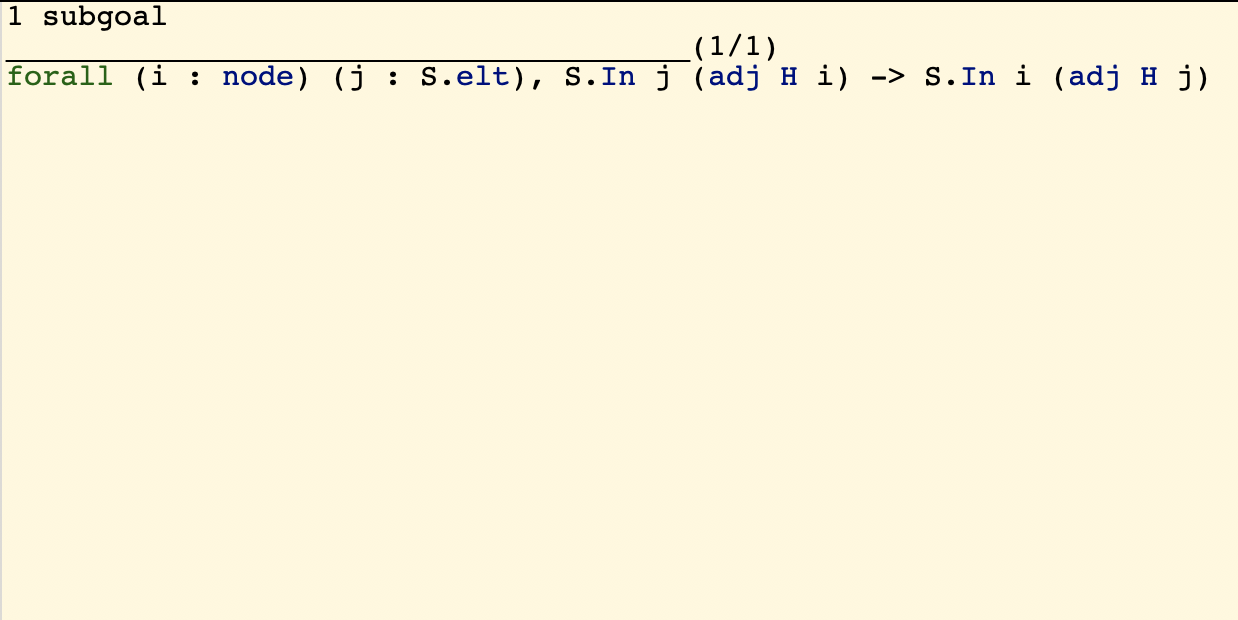
\includegraphics[width=1\linewidth]{context4.png}}
  \end{minipage}
\end{figure}
\end{frame}

\begin{frame}[fragile]
\frametitle{Доказательства корректности \\ операций над графами: {\tt H\_ok}}

\begin{figure}[h]
  \begin{minipage}[h]{1\linewidth}
    \center{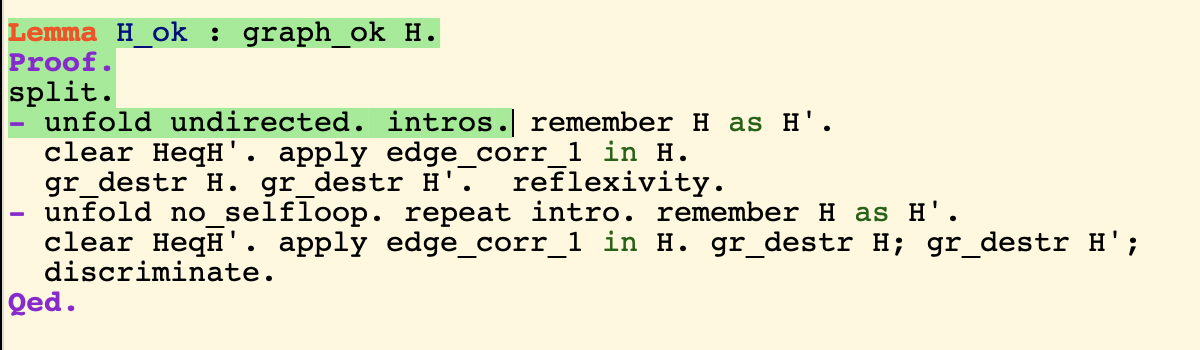
\includegraphics[width=1\linewidth]{H-ok5.png}}
  \end{minipage}
  \begin{minipage}[h]{1\linewidth}
    \center{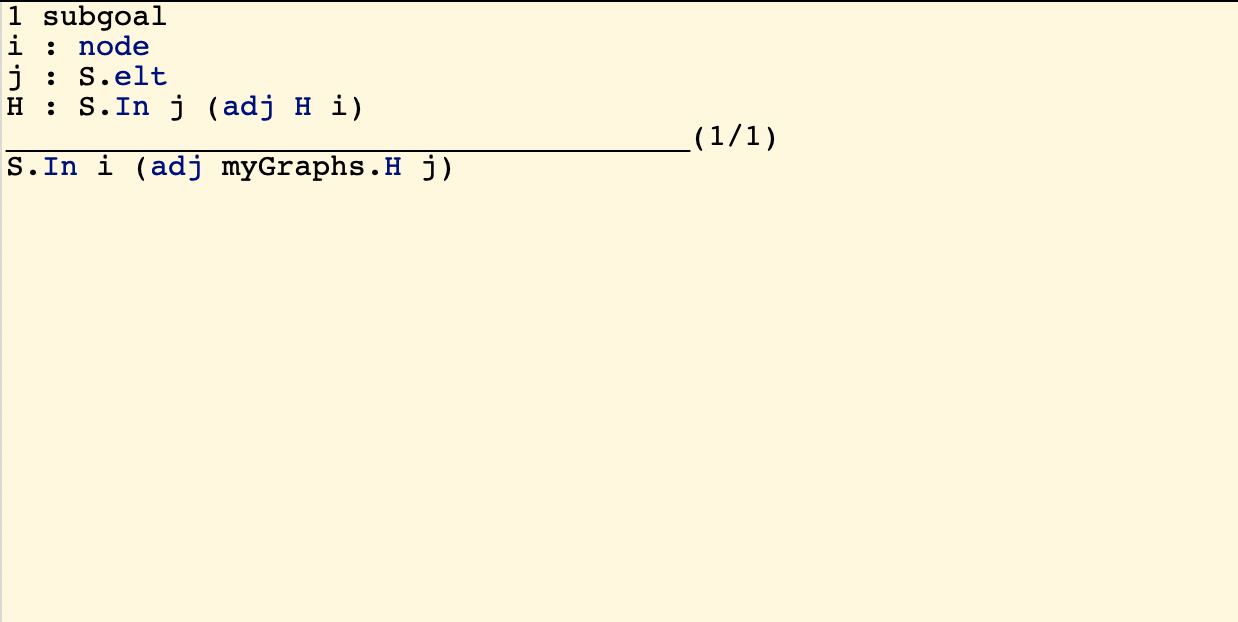
\includegraphics[width=1\linewidth]{context5.png}}
  \end{minipage}
\end{figure}
\end{frame}

\begin{frame}[fragile]
\frametitle{Доказательства корректности \\ операций над графами: {\tt H\_ok}}

\begin{figure}[h]
  \begin{minipage}[h]{1\linewidth}
    \center{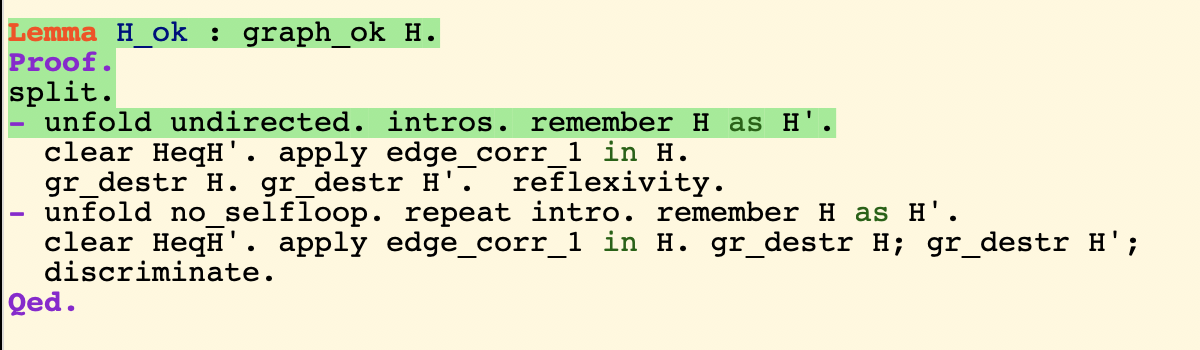
\includegraphics[width=1\linewidth]{H-ok6.png}}
  \end{minipage}
  \begin{minipage}[h]{1\linewidth}
    \center{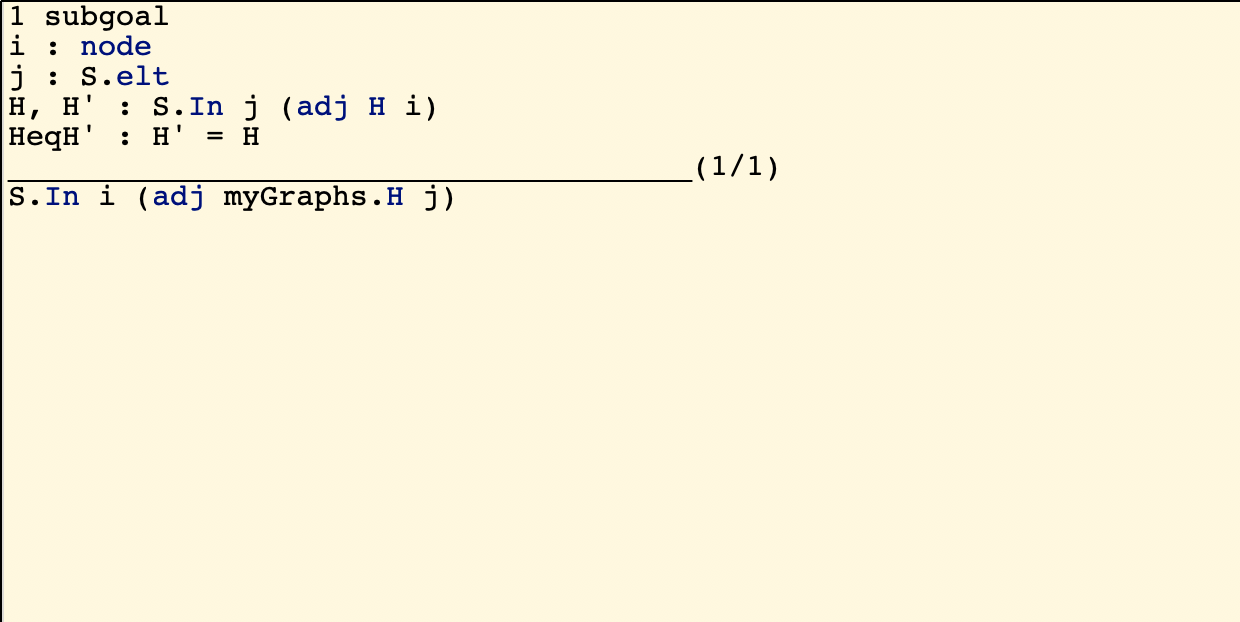
\includegraphics[width=1\linewidth]{context6.png}}
  \end{minipage}
\end{figure}
\end{frame}

\begin{frame}[fragile]
\frametitle{Доказательства корректности \\ операций над графами: {\tt H\_ok}}

\begin{figure}[h]
  \begin{minipage}[h]{1\linewidth}
    \center{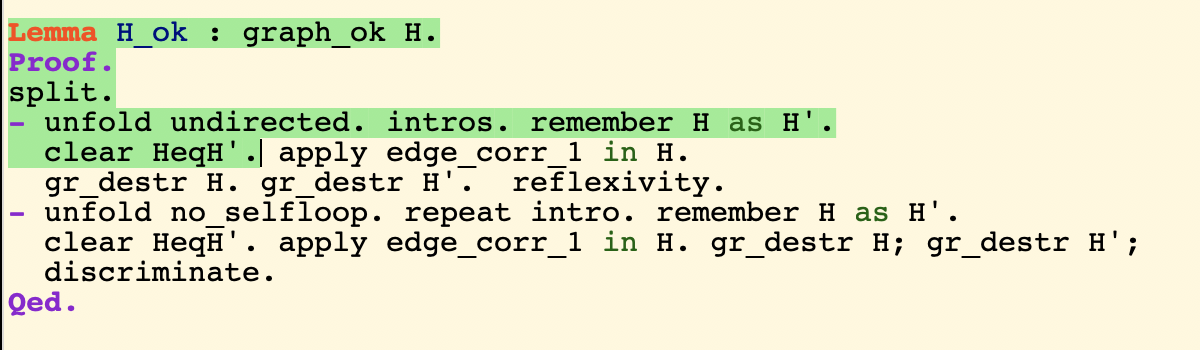
\includegraphics[width=1\linewidth]{H-ok7.png}}
  \end{minipage}
  \begin{minipage}[h]{1\linewidth}
    \center{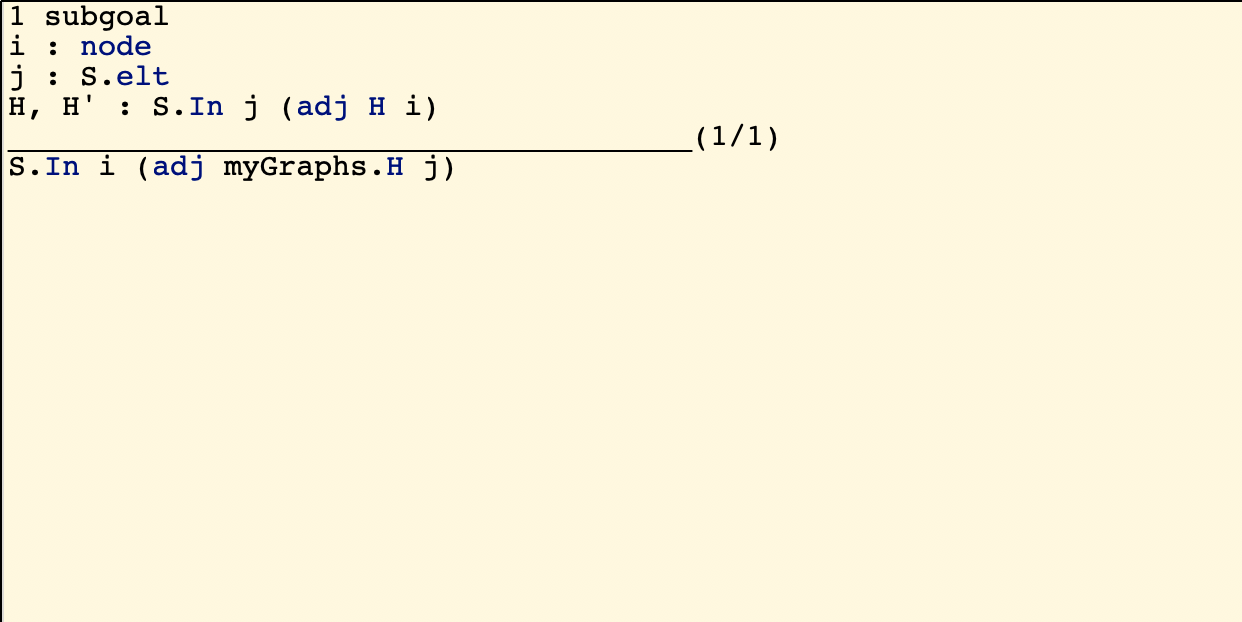
\includegraphics[width=1\linewidth]{context7.png}}
  \end{minipage}
\end{figure}
\end{frame}

\begin{frame}[fragile]
\frametitle{Доказательства корректности \\ операций над графами: {\tt H\_ok}}

\begin{figure}[h]
  \begin{minipage}[h]{1\linewidth}
    \center{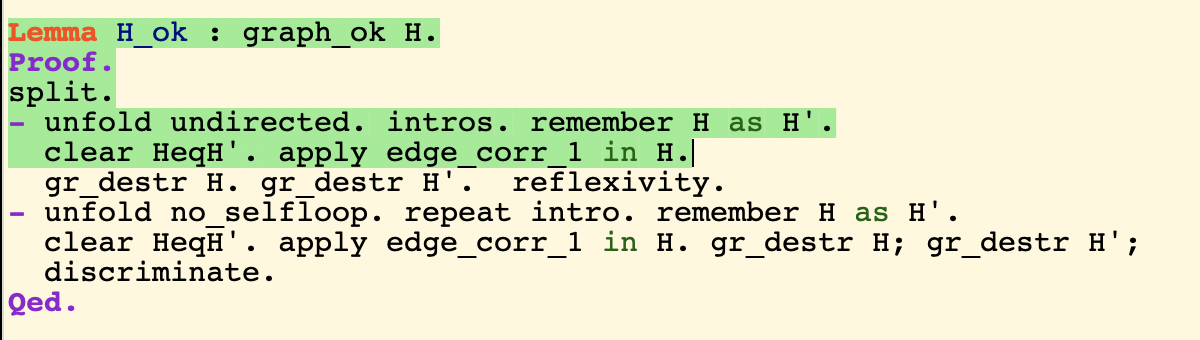
\includegraphics[width=1\linewidth]{H-ok8.png}}
  \end{minipage}
  \begin{minipage}[h]{1\linewidth}
    \center{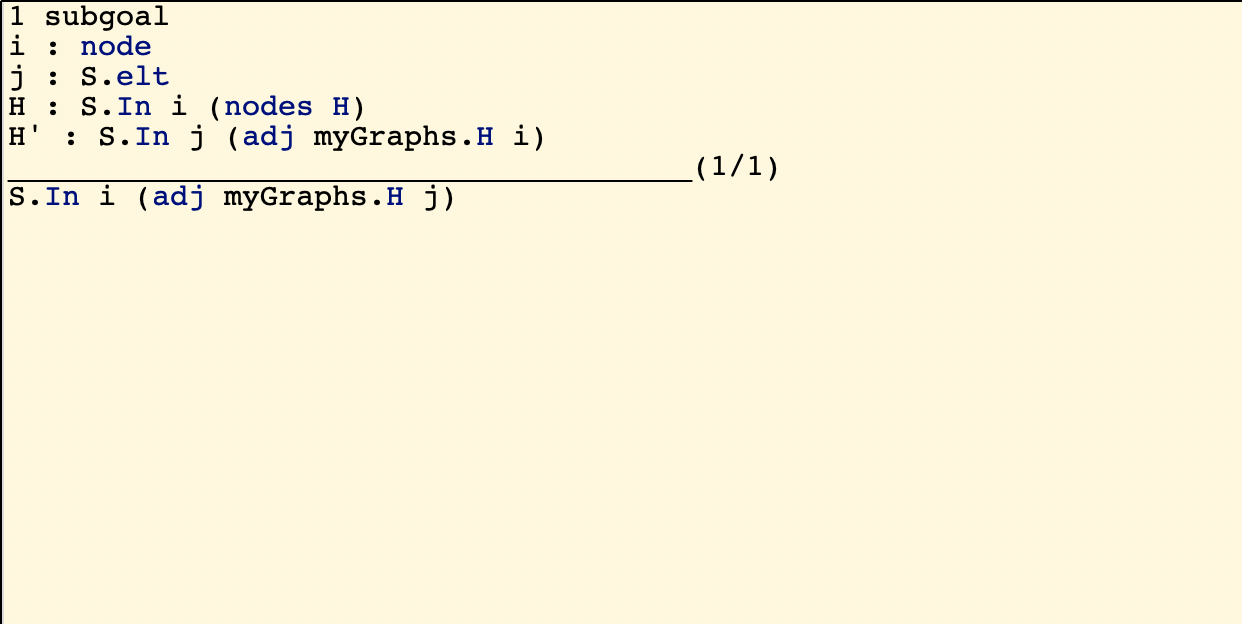
\includegraphics[width=1\linewidth]{context8.png}}
  \end{minipage}
\end{figure}
\end{frame}

\begin{frame}[fragile]
\frametitle{Доказательства корректности \\ операций над графами: {\tt H\_ok}}

\begin{figure}[h]
  \begin{minipage}[h]{1\linewidth}
    \center{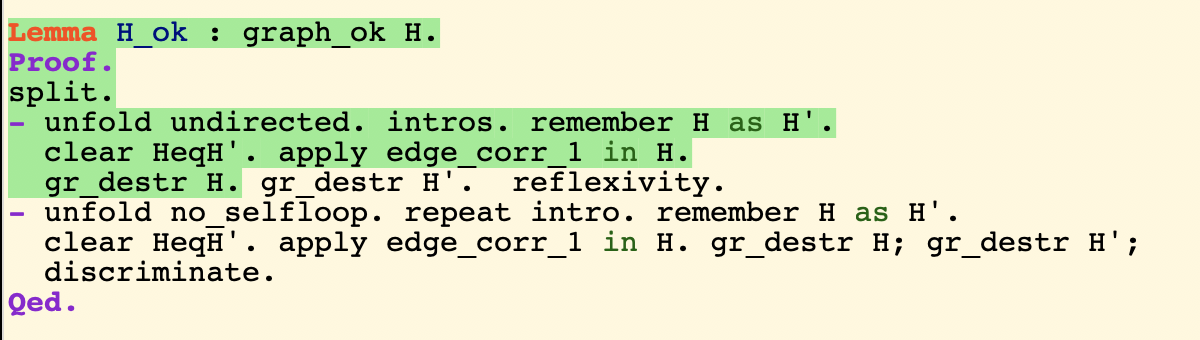
\includegraphics[width=1\linewidth]{H-ok9.png}}
  \end{minipage}
  \begin{minipage}[h]{1\linewidth}
    \center{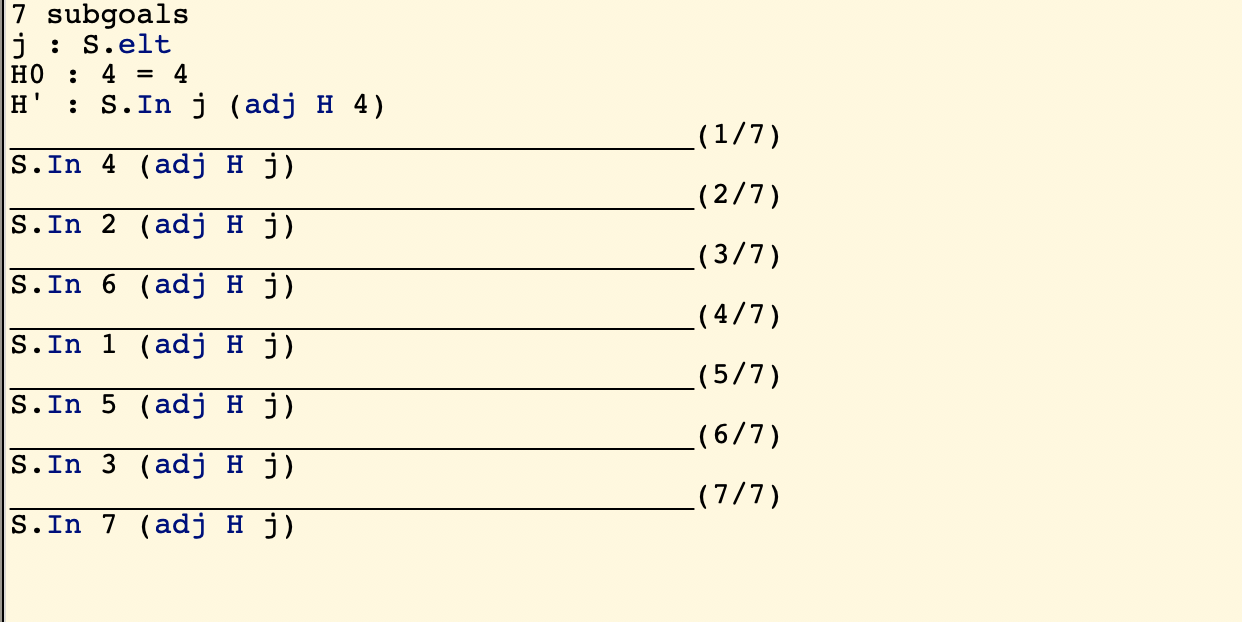
\includegraphics[width=1\linewidth]{context9.png}}
  \end{minipage}
\end{figure}
\end{frame}

\begin{frame}[fragile]
\frametitle{Доказательства корректности \\ операций над графами: {\tt H\_ok}}

\begin{figure}[h]
  \begin{minipage}[h]{1\linewidth}
    \center{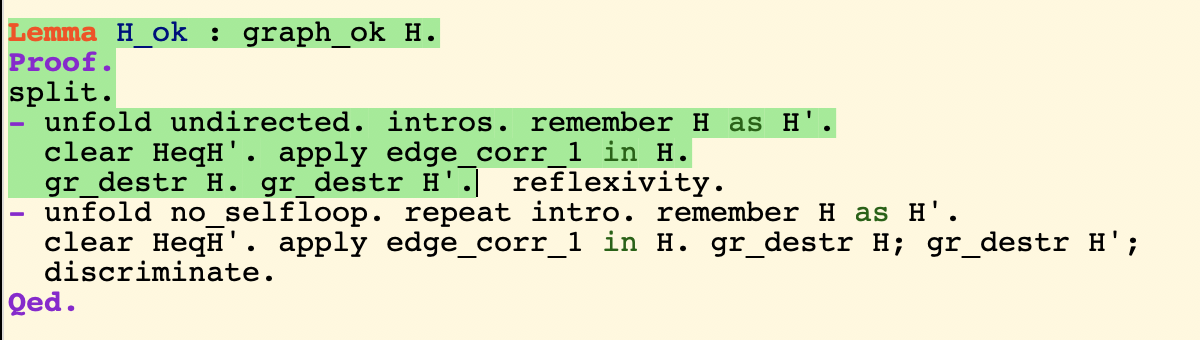
\includegraphics[width=1\linewidth]{H-ok10.png}}
  \end{minipage}
  \begin{minipage}[h]{1\linewidth}
    \center{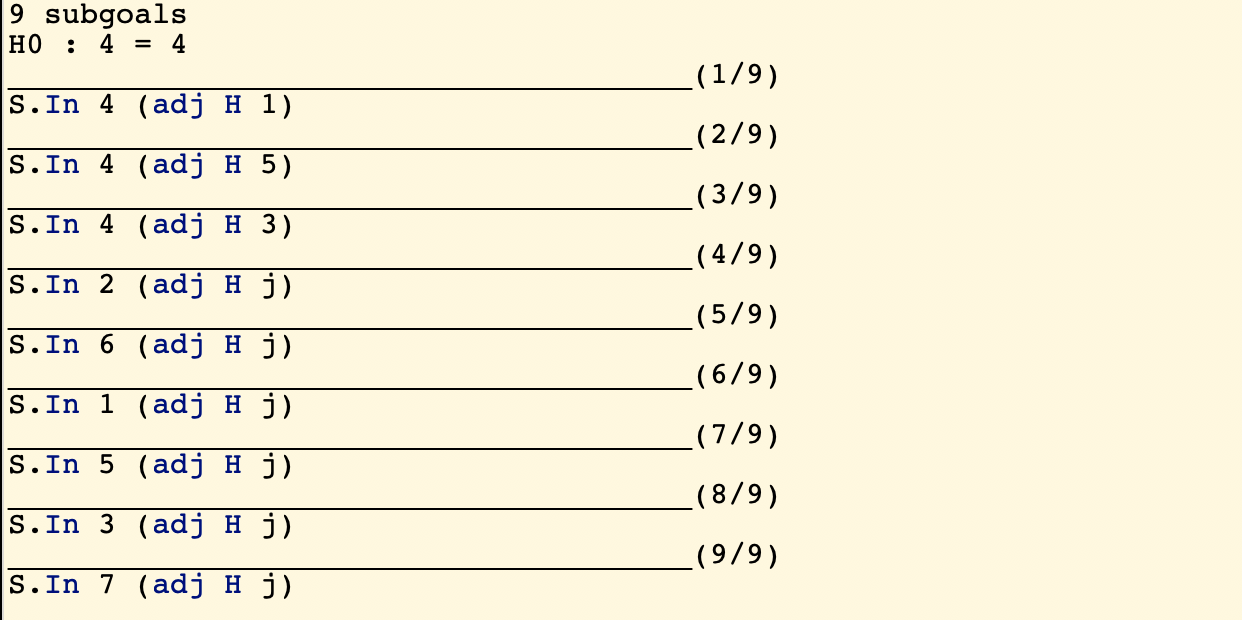
\includegraphics[width=1\linewidth]{context10.png}}
  \end{minipage}
\end{figure}
\end{frame}

\begin{frame}[fragile]
\frametitle{Доказательства корректности \\ операций над графами: {\tt H\_ok}}

\begin{figure}[h]
  \begin{minipage}[h]{1\linewidth}
    \center{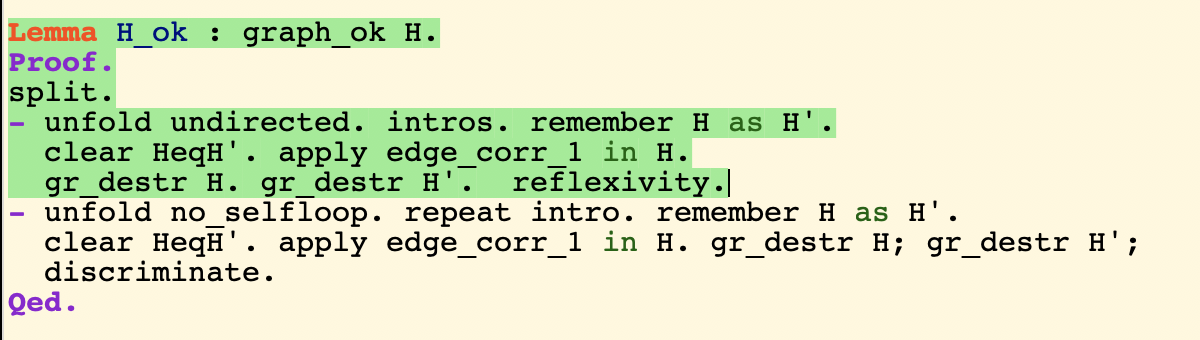
\includegraphics[width=1\linewidth]{H-ok11.png}}
  \end{minipage}
  \begin{minipage}[h]{1\linewidth}
    \center{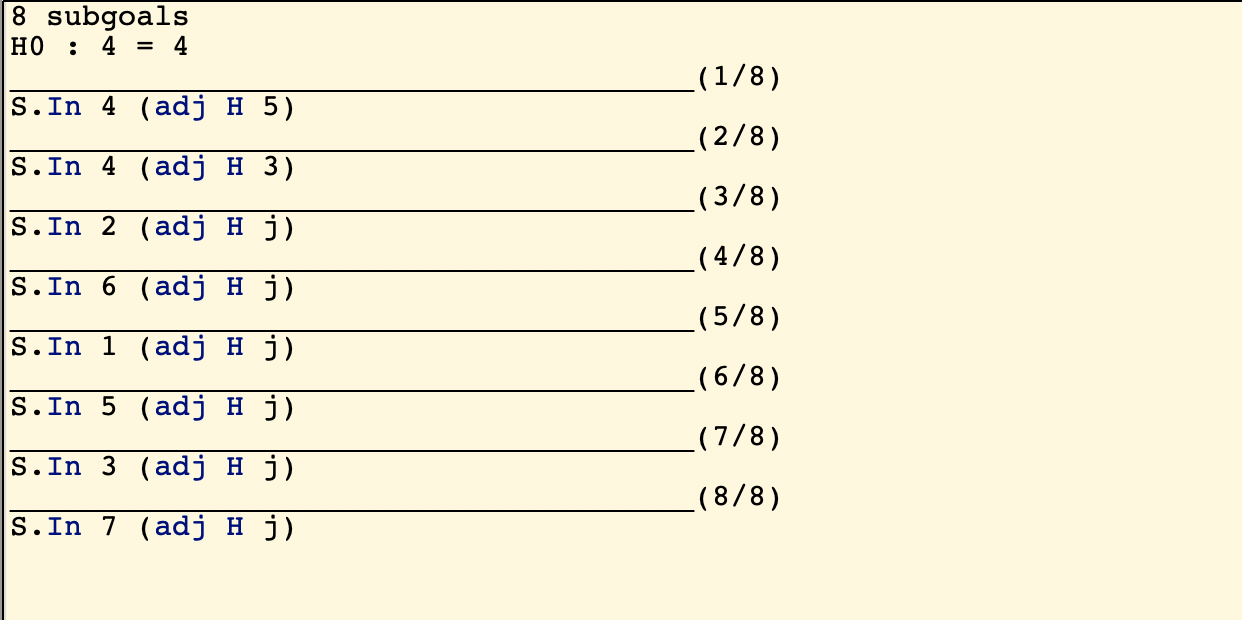
\includegraphics[width=1\linewidth]{context11.png}}
  \end{minipage}
\end{figure}
\end{frame}

\begin{frame}[fragile]
\frametitle{Доказательства корректности операций над графами: тактика {\tt gr\_destr}}

\begin{verbatim}
Ltac gr_destr h := 
  apply S.elements_1 in h; compute in h;
  repeat rewrite InA_cons in h;
  rewrite InA_nil in h;
  repeat destruct h as [? | h]; 
  try inversion h; subst.
\end{verbatim}
\end{frame}


\begin{frame}[fragile]
\frametitle{Теорема о корректности \\ добавления ребра }

{\small 
\begin{verbatim}
Lemma add_edge_corr' : forall g x y a b,
  edge (add_edge (a, b) g) x y <-> edge g x y \/
  (x = a /\ y = b) \/ (x = b /\ y = a).
\end{verbatim}

\begin{verbatim}
Lemma add_edge_corr : forall g a b, graph_ok g -> 
  a <> b -> graph_ok (add_edge (a, b) g).
\end{verbatim} }

\end{frame}

\begin{frame}
\frametitle{Типы возможных правильных раскрасок графа {\tt T} в не более чем 4 цвета}
\begin{figure}[H]
  \center
  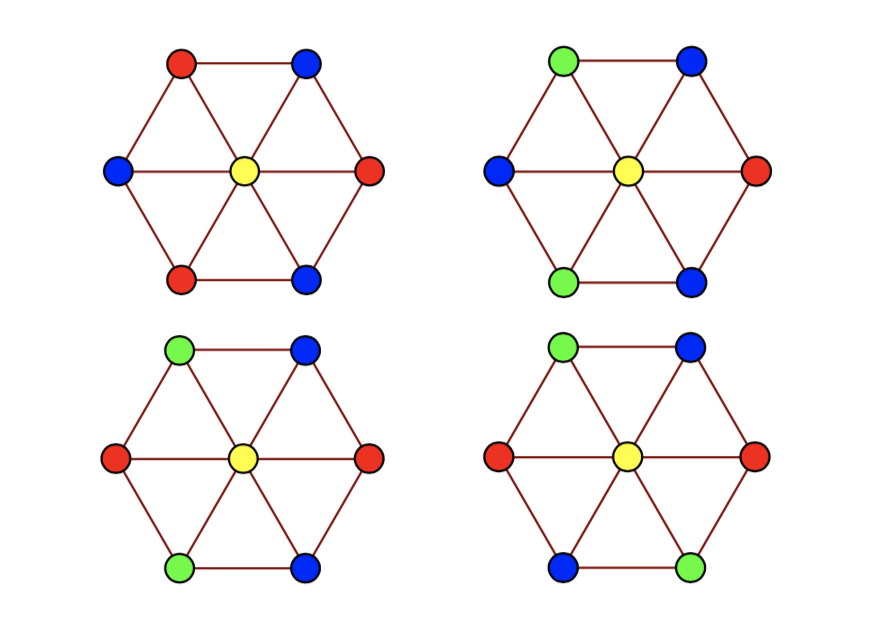
\includegraphics[width=0.75\linewidth]{Colorings_of_H.png}
\end{figure}
\end{frame}


\begin{frame}[fragile]
\frametitle{Типы возможных правильных раскрасок графа {\tt T} в не более чем 4 цвета}
{\footnotesize
\begin{verbatim}
Definition Coloring := positive -> positive.

Inductive is_color : positive -> Prop :=
| c1: is_color 1
| c2: is_color 2
| c3: is_color 3
| c4: is_color 4.

Definition is_coloring (c : Coloring) :=
    forall x : positive, is_color (c x).

Definition is_good_coloring (c : Coloring) (g : graph) :=
  is_coloring c /\ forall x y : positive, 
    S.In y (adj g x) -> c x <> c y.
\end{verbatim}
}
\end{frame}

\begin{frame}[fragile]
\frametitle{Типы возможных правильных раскрасок графа {\tt T} в не более чем 4 цвета}
{\footnotesize
\begin{verbatim}
Lemma coloring_H:
  forall c: Coloring, is_good_coloring c H ->
  type1_H c \/ type2_H c \/ type3_H c \/ type4_H c.
Proof.
  intros. unfold is_good_coloring in H. 
  unfold is_coloring in H. destruct H.
  color_next H 1;
    color_next H 2; try find_contr H0 c;
      color_next H 3; try find_contr H0 c;
        color_next H 4; try find_contr H0 c;
          color_next H 5; try find_contr H0 c;
            color_next H 6; try find_contr H0 c;
              color_next H 7; try find_contr H0 c;
                find_type H3 H5 H7 H9 H11 H13 H15 c.
Qed.
\end{verbatim} }
\end{frame}

\begin{frame}
\frametitle{Результаты и выводы}
\begin{itemize}
    \item Разработаны эффективные методы конструирования графов, обладающих высокой степенью симметрии
    \item Эти методы применены к графам {\tt H}, {\tt J}, {\tt K} и {\tt L}
    \item Разработаны методы работы с раскрасками графов
    \item Верифицировано доказательство того, что существует ровно 4 существенно различные раскраски графа {\tt H} в не более чем 4 цвета
\end{itemize}
\end{frame}

\begin{frame}
\frametitle{Планы будущей работы}
\begin{itemize}
    \item Формализация алгоритма раскраски графа из статьи де Грея
    \item Верификация указанного алгоритма
    \item Формализация конструкций графов из главы $4$, основывающихся на реализации на плоскости 
\end{itemize}
\end{frame}

\begin{frame}
\begin{center}
{\color{purple}{Спасибо за внимание!}}
\end{center}
\end{frame}

\end{document} 